\documentclass[a4paper]{jsarticle}
\usepackage{bm}
\usepackage[dvipdfmx]{graphicx}
\usepackage{amsmath,amsfonts}
\usepackage{cite}
\usepackage{physics}
\usepackage[version=4]{mhchem}
\usepackage{comment}
\usepackage{float}
\usepackage[compatibility=false, font=small, labelfont=bf, labelsep=quad]{caption} % 設定を明示
\usepackage{url}
\newcommand{\diff}{\mathrm{d}}
\title{有限温度における\ce{Sn}核の超流動相転移解析\\Woods-Saxonポテンシャルとseniority pairingモデルの応用}
\author{千葉大学理学部物理学科\\
21S2008K 根岸颯}
\date{2025年2月}
\begin{document}
\maketitle
\newpage

\tableofcontents
\newpage
\section{序論}
原子核におけるenergy scaleは1MeV$\simeq10^{10}$K程度であり、
地上でこのような熱平衡状態が実現されるとは考えられず、
実際に通常扱う原子核は$T=0$にあると見なしても問題は生じない。
しかし、恒星内部やその終焉時の極限環境下においては原子核においては
有限温度の熱浴の下にあると考える事ができる。
また、"核温度"と呼ばれる孤立した原子核の励起状態の統計的性質を調べるための概念も存在する。
有限温度の原子核の性質も様々な場面に対して応用が期待される重要な概念である。
ここでは\ce{{}^{100	-132}Sn}核を例に取り、Woods-Saxon potentialとseniority modelを用いた理解を試みる。

\section{理論}
\subsection{3次元極座標調和振動子}\label{sec.3dim}
本解析では、3次元極座標調和振動子の波動関数にスピンを含めた基底$\ket{i}=\psi_{n\ell m}\ket{s} \ (s=\pm1)$を採用する。
potentialについては中心力potentialを採用するため、角度方向の波動関数は省略する。
このセクションでは主に文献\cite{qm_a.pdf}を参考にした。
中心力ポテンシャル$V(r)$内でのSchr\"{o}dinger方程式は、
\begin{equation}
  H\psi(\bm{r})=E\psi(\bm{r}),\qquad H=\dfrac{\bm{p}^2}{2M} + V(\bm{r}),\quad\bm{p}=-i\hbar\nabla
  \label{3dim}
\end{equation}
であり、計算の結果により$r\neq0$のとき
$\nabla^2 = \dfrac{1}{r}\dfrac{\partial^2}{\partial r^2}r-\dfrac{1}{r^2}\bm{L}^2$
と表されるので、ハミルトニアンを書き直すと、
\begin{equation}
  H = H_r + \dfrac{\hbar^2\bm{L}^2}{2Mr^2},\qquad H_r = -\dfrac{\hbar^2}{2M}\dfrac{1}{r}\dfrac{\partial^2}{\partial r^2}r +V(\bm{r})
\end{equation}
であり、このように書くと分かる通り、$\comm{H}{\bm{L}}=0$である。
整理すると、$H,\bm{L}^2,L_z$の同時固有状態が存在する。
$\bm{L}^2,L_z$の同時固有状態関数は球面調和関数$Y_{\ell m}(\theta,\phi)$であるから、
$H,\bm{L}^2,L_z$の同時固有状態$\psi(\bm{r}) $は、
\begin{equation}
  \psi(\bm{r})=R(r)Y_{\ell m}(\theta,\phi),\qquad m=\ -\ell,-\ell+1,\cdots,\ell-1,\ell
\end{equation}
と書くことができる。このときの$R(r)$の取り方によらず、$\psi(\bm{r})$は$\bm{L}^2,L_z$の固有状態であるから、
$\psi(\bm{r})$が$H$の固有状態になるように$R(r)$を決定する。
$\bm{L}^2Y_{\ell m}(\theta,\phi)=\ell(\ell+1)Y_{\ell m}(\theta,\phi)$より、
$H\psi(\bm{r})=E\psi(\bm{r})$は
\begin{equation}
  \left(-\dfrac{\hbar^2}{2M}\dfrac{1}{r}\dfrac{d^2}{d r^2}r+ \dfrac{\hbar^2\ell(\ell+1)}{2Mr^2}+V(r)\right)R_\ell (r)=ER_\ell (r)
\end{equation}
と書く事ができる。式から$E$と$R(r)$が決まり、$\ell$には依存するが$m$には依存しないことがわかる。
両辺に$r$をかけると、$u_\ell(r)=rR_\ell(r)$と表せるため、
\begin{equation}
  \left(-\dfrac{\hbar^2}{2M}\dfrac{d^2}{d r^2}+ \dfrac{\hbar^2\ell(\ell+1)}{2Mr^2}+V(r)\right)u_\ell(r)=Eu_\ell(r)
  \label{1dim}
\end{equation}
と表すことができ、
これはポテンシャルが$U_\ell(r)=\dfrac{\hbar^2\ell(\ell+1)}{2Mr^2}+V(r)$である$r\ge0$の
1次元Schr\"{o}dinger方程式である。\par
調和振動子の場合には、$V(r)=\dfrac{M\omega^2r^2}{2}$であるため、式(\ref{1dim})は、
\begin{equation}
  \left(\dfrac{\diff^2}{\diff q^2} -\dfrac{l(l+1)}{q^2} -q^2+\dfrac{2E}{\hbar\omega}\right)
  u_\ell(q)=0,\quad\text{ただし}\ q=\alpha r,\ \alpha=\sqrt{\dfrac{M\omega}{\hbar}}
\label{3h.o. eq}
\end{equation}
になる。波動関数の境界条件などを考えれば、
$u_\ell(q)=f(q)v_{\ell}(q),f(q)=q^{\ell+1}e^{-q^2/2}$と置くことができ、これを用いて式(\ref{3h.o. eq})を計算すれば、
\begin{equation}
  \dfrac{d^2v_{\ell}}{dq^2}+\dfrac{2}{f}\dfrac{df}{dq}\dfrac{dv_{\ell}}{dq}+
  \left(
    \dfrac{1}{f}\dfrac{d^2f}{dq^2}-\dfrac{\ell(\ell+1)}{q^2}-q^2+\dfrac{2E}{\hbar\omega}
  \right)v_\ell=0
\end{equation}
である。$\dfrac{df}{dq}$や$\dfrac{d^2f}{dq^2}$の計算自体は単純であるので代入すれば、
\begin{equation}
  \dfrac{d^2v_{\ell}}{dq^2}+2\left(\dfrac{\ell+1}{q}-q\right)\dfrac{dv_{\ell}}{dq}
  -\left(2\ell + 3 - \dfrac{2E}{\hbar\omega}\right)v_\ell=0
  \label{v_ell}
\end{equation}
ここで$\rho=q^2$と変数変換を行えば、
\begin{equation}
  \dfrac{d}{dq}=\dfrac{d\rho}{dq}\dfrac{d}{d\rho}=2\sqrt{\rho}\dfrac{d}{d\rho},\quad
  \dfrac{d^2}{dq^2}=4\sqrt{\rho}\dfrac{d}{d\rho}\sqrt{\rho}\dfrac{d}{d\rho}
    =4\left(\rho\dfrac{d^2}{d\rho^2}+\dfrac{1}{2}\dfrac{d}{d\rho}\right)
\end{equation}
であるから、これを用いて式(\ref{v_ell})を書き換えれば、
\begin{equation}
  \rho\dfrac{d^2v_{\ell}}{d\rho^2} +
  \left(\ell+\dfrac{3}{2}-\rho\right)\dfrac{dv_{\ell}}{dq} -\alpha v_{\ell}=0,\qquad
  \alpha \equiv \dfrac{1}{2}\left(\ell +\dfrac{3}{2} -\dfrac{E}{\hbar\omega}\right)
\end{equation}
これは、$a,b$を任意定数とした合流型超幾何微分方程式
\begin{equation}
  \left(x\dfrac{d}{dx^2}+(b-x)\dfrac{d}{dx}-a\right)w(x)=0\qquad
  b\neq -n,n=0,1,2,\cdots
\end{equation}
において、$a=\alpha,b=\ell+\dfrac{3}{2}$とした時の解と一致する。そのため$u_\ell(0)=0$を満たす解は、
合流型超幾何関数$M(a,b,x)$を用いて
\begin{equation}
  u_\ell(q) = Cq^{\ell+1}e^{-q^2/2}M(\alpha,\ell+3/2,q^2)
\end{equation}
になる。このとき$\alpha=-n=0,-1,-2,\cdots$のとき、$u_\ell(q)\xrightarrow{q\rightarrow\infty}0$
になるため、エネルギー固有値は、
\begin{equation}
  E_{nl}=\hbar\omega\left(2n+\ell+\dfrac{3}{2}\right)
\end{equation}
求めることができる。\par
以上のことから波動関数$\psi_{n\ell m}$は、
\begin{equation}
  \psi_{n\ell m}(\bm{r})=\dfrac{u_{n\ell}(r)}{r}Y_{\ell m}(\theta,\phi),\quad 
  u_{n\ell}(q) = A_{n\ell}\ q^{\ell+1}e^{-q^2/2}M(-n,\ell+3/2,q^2)
\end{equation}
である。ただし、$q=a r =\sqrt{\dfrac{M\omega}{\hbar}} r$である。
規格化条件は$\rho=q^2$とすると
\begin{equation*}
  \dfrac{A_{n\ell}^2}{2a}\int_{0}^{\infty}d\rho\rho^{\ell+1/2}e^{-\rho}
  \left(M(-n,\ell+3/2,\rho)\right)^2=1
\end{equation*}
である。このときの$A_{n\ell}$の値は、
\begin{equation}
  A_{n\ell}=\sqrt{2a\dfrac{\varGamma(\ell+n+3/2)}{n!(\varGamma^2(\ell+3/2))}}
\end{equation}
である。$n$は$u_{n\ell}(r)$の節(ノード)の個数である。\par
今回の問題設定では球対称ポテンシャル下での粒子状態を求めているため、動径方向の波動関数である
\begin{equation}
  u_{n\ell}(q) = \sqrt{2a\dfrac{\varGamma(\ell+n+3/2)}{n!(\varGamma^2(\ell+3/2))}}q^{\ell+1}e^{-q^2/2}M(-n,\ell+3/2,q^2)
\end{equation}
を計算に用いる。ただし、$q=ar,a=\sqrt{\dfrac{M\omega}{\hbar}}$である。

\subsection{Woods-Saxon potentialとLS相互作用}\label{sec.ws}
\ref{sec.3dim}では簡単なmodelとして調和振動子モデルを用いたが、
このpotentialでは原子核のmagic numberに代表される特徴的な性質を十分に記述できない。
しかしながら2体以上の相互作用をpotentialに含めてしまうとやや複雑になりすぎてしまう。
そのため、potentialを簡単にするために、それぞれの粒子が独立に運動しているとして平均場近似を行う。
この際、調和振動子モデルよりも正確に特徴を捉えることができる
Woods-Saxon potentialとLS(スピン軌道)相互作用を導入する。
このセクションでは主に文献\cite{nucleus_structure},\cite{nucleus.pdf}を参考にした。\par
Woods-Saxon potentialは調和振動子モデルで異なる$\ell$の状態が縮退しているという部分を解決した。
具体形を以下に示す。
\begin{equation}
  V_{\text{WS}}(r)=\dfrac{u_{0}}{1+\exp((r-R)/a)},\ u_{0}=\left(-51+33\dfrac{N-Z}{A}\right)
  \label{WSpt}
\end{equation}
ここで$a=0.67$fm,$R=r_0A^{1/3},r_0=1.27$fmである。
このpotentialを用いることで、異なる$\ell$の状態の縮退が完全に解ける。その数値計算の結果を下に示す。
\begin{figure}[H]
  \centering
  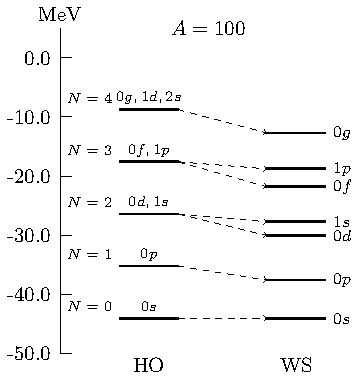
\includegraphics[width=.5\textwidth]{main_fig/HOvsWS.pdf}
  \captionsetup{width=0.8\textwidth}
  \caption{核子数 $A=100$ のときの調和振動子 (HO) モデル (右側) と 
  Woods-Saxon potential (WS) (左側) の比較。\\
  ただし、$N = 2n + \ell$ 。
  また$0s$や$1p$などは固有状態$n\ell$を表現していて$\ell=0,1,2,\cdots$に対して$s,p,d,f,g,\cdots$が対応する。}
  \label{fig:HOvsWS}
\end{figure}
このポテンシャルの設定では$\ell$の縮退は完全に解けているが、それぞれの核子のスピンは
考慮できていない。そうした問題を解決するために
1949年、MayerとJansenはそれぞれ独立に、スピン軌道力(LS相互作用)がポテンシャルに
含まれているとすれば、様々な魔法数を説明することができることを発見した。
このときに導入したポテンシャル$U(r)$は、
\begin{equation}
  U(r)=V(r)+\lambda_{\ell s}\dfrac{1}{r}\dfrac{\partial V}{\partial r}\bm{\ell}\cdot\bm{s}
\end{equation}
と表される。ここで、$\bm{\ell}\cdot\bm{s}$について考えるが、全角運動量$\bm{j}=\bm{\ell}+\bm{s}$
を用いれば$\bm{j},\bm{\ell},\bm{s}$を用いて$2\bm{\ell}\cdot\bm{s}=\bm{j}^2-\bm{\ell}^2-\bm{s}^2$
であるから、$\bm{j}^2,\bm{\ell}^2,\bm{s}^2$の同時固有状態であれば$H$の固有状態となる。
つまり波動関数は、$\ket{i}=\psi_{n\ell m}\ket{s}(s=\pm1)$であれば良い。
このとき、$\bm{j}^2,\bm{\ell}^2,\bm{s}^2$の固有値はそれぞれ、
\begin{equation}
  \quad\bm{\ell}^2\ket{i}=\ell_{i}(\ell_{i}+1)\ket{i}
  \quad\bm{s}^2\ket{i}=\dfrac{1}{2}\left(\dfrac{1}{2}+1\right)\ket{i}
  \quad\bm{j}^2\ket{i}=j_{i}(j_{i}+1)\ket{i}
\end{equation}
と表現される。ただし$j=\ell\pm1/2$である。
以上のことから、LS相互作用の大きさ$V_{\ell j}$は
\begin{equation}
  V_{\ell j}=\dfrac{1}{2}\left(
    j(j+1)-\ell(\ell+1)-\dfrac{3}{4}
  \right)
  =\left\{
    \begin{alignedat}{2}
      \ &\dfrac{\ell}{2},\quad&j=\ell+\dfrac{1}{2}\\
      \ &-\dfrac{\ell+1}{2},\quad&j=\ell-\dfrac{1}{2}
    \end{alignedat}
  \right.
\end{equation}
となるから、異なるスピンの値でエネルギー固有値が分離することが確認できた。
また、それぞれの状態は固有状態$n\ell$に付け加えて$n\ell_{j}$で指定される。
また、このときそれぞれの軌道に入る陽子または中性子の数は$2j+1$個である。
例として$0s_{1/2}$軌道には $2(1/2)+1=2$個、$0g_{9/2}$軌道には $2(9/2)+1=10$個の陽子または中性子が入る。

以上のことから固有状態が$n,\ell,j$で指定されることが確認できた。よってSchr\"{o}dinger方程式は、
\begin{equation}
  H\ket{i}=\left(\dfrac{\bm{p}^2}{2M} + V_{\text{WS}}(\bm{r})+a_{\ell s}V_{\ell j}\right)\ket{i}=E\ket{i}
\end{equation}
と表されることがわかった。$a_{\ell s}$は$a_{\ell s}=22-14(N-Z)/A$として与えられる。


本研究で用いるハミルトニアン$H=\bm{p}^2/2M+U(r)$で、
\begin{equation}
  U(r)=u_0f(r)+u_{ls}r_0^2\dfrac{1}{r}\dfrac{df(r)}{dr}\boldsymbol{\ell\cdot s}+U_{Coul}(r)\dfrac{1-\tau}{2},\quad f(r)=\dfrac{1}{1+\exp((r-R)/a)}
  \label{Hamiltonian}
\end{equation}
ただし、$r_0=1.27\text{fm},R=r_0A^{1/3}\text{fm},a=0.67\text{fm}$であり、
ポテンシャルの係数$u_0,u_{\ell s}$の値は$u_0=-51+33(N-Z)/A,u_{\ell s}=22-14(N-Z)/A$を採用した\cite{nucleus_structure}。
$U_{Coul}(r)$は半径$R$の一様帯電球の与えるpotentialで近似し、アイソスピンの$z$成分$\tau$によって
陽子($\tau=-1$)と中性子($\tau=+1$)を区別する。

この方程式を数値的に解いたものを下に示す。
実際に魔法数をうまく表現できていることが確かめられる。
\begin{figure}[H]
  \centering
  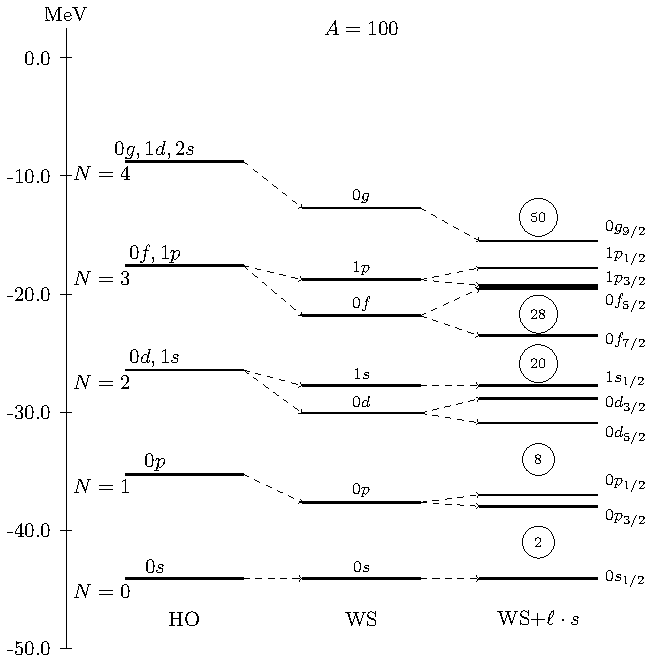
\includegraphics[width=.8\textwidth]{main_fig/tot.pdf}
  \captionsetup{width=0.8\textwidth}
  \caption{核子数 $A=100$ のときの比較。\\調和振動子 (HO) モデル (右側), 
  Woods-Saxon potential (WS) (中央),
  WSとLS相互作用(右側)の比較。}
  \label{fig:HOvsWSvsls}
\end{figure}

\subsection{seniority pairing}\label{sec.seniority}
ペアリング相互作用は核子間の相互作用の短距離部分によるものであり、
特にseniority pairingは($I=0$)に結合したペアが影響を受ける最も単純なペアリングモデルの1つである。
このセクションは\cite{thenuclearmanybody}を参考にした。
seniority pairingを採用した時のハミルトニアンは
$\epsilon_j$を(\ref{Hamiltonian})で求めた単粒子エネルギーとして
\begin{equation}
  H=\sum_{j}\epsilon_jN_j -gS_+S_-;\quad S_+\equiv\sum_j S_{j+},S_-\equiv(S_+)^{\dagger}
\end{equation}
と与えられる。$S_{j+}$は$j$に対するquasi-spin operatorである。\par
quasi-spin operatorは生成消滅演算子$a_j^\dagger,a_j$を用いて以下のように定義され、
\begin{align}
  S_{j+}=a_j^\dagger a_{-j}^\dagger\\
  S_{j-}=a_{-j} a_{j}\\
  S_0 = \dfrac{1}{2}\left(a_j^\dagger a_{j} +a_{-j}^\dagger a_{-j} - 1\right)
\end{align}
これらは以下の角運動量交換関係を満たす。
\begin{align*}
  \comm{S_{j+}}{S_{j-}}&=2S_0\\
  \comm{S_0}{S_{j+}}&=S_{j+}\\
  \comm{S_0}{S_{j-}}&=-S_{j-}.
\end{align*}
ここではペアリングによるエネルギー変化には注目せず、
BCS理論を用いてペアリングの強さである$g$の値を決定し原子核の相転移について
考えていく。
\subsection{BCS理論}
\subsubsection{絶対零度の場合}
\subsubsection{有限温度の場合}
\section{手法}
\section{結果と考察}
\section{結論}

\bibliographystyle{plain}
\bibliography{list}
\section{付録}
\subsection{合流型超幾何関数周辺}
\end{document}
